\begin{center}
\Huge
	Bestemte integraler ved substitution		
\end{center}

\section*{Bestemte integraler ved substitution}
\stepcounter{section}

Skal vi bestemme bestemte integraler ved substitution er fremgangsmåden først at bestemme en stamfunktion ved substitution og efterfølgende at indsætte grænserne i stamfunktionen som vi kender det fra sædvanlige bestemte integraler. Lad os betragte et eksempel.

\begin{exa}
	Vi ønsker at bestemme værdien af integralet
	\begin{align*}
		\int_0^2(4t+8)e^{t^2+4t} dt.
	\end{align*}
	Vi sætter den indre funktion $u$ til at være $u = t^2 + 4t$ og får
	\begin{align*}
		\frac{du}{dt} = 2t + 4 \ \Leftrightarrow	\ \frac{du}{2t+4} = dt. 
	\end{align*}
	Vi laver nu substitutionen for det ubestemte integral
	\begin{align*}
		\int (4t + 8)e^{t^2 + 4t} dt &= \int (4t + 8)e^u \frac{du}{2t+4} \\
		&=\int 2(2t + 4)e^u \frac{du}{2t + 4} \\
		&= \int 2e^u du \\
		&= 2e^u + k \\
		&= 2e^{t^2+4t} + k
	\end{align*}
	Vi kan bruge denne stamfunktion til at bestemme det bestemte integral.
	\begin{align*}
		\int_0^2(4t+8)e^{t^2+4t} dt &= \left[ 2e^{t^2+4t} \right]_0^2 \\
		&=\underbrace{2e^{2^2+4\cdot 2}}_{=F(2)} - \underbrace{2e^{0^2+4\cdot 0}}_{=F(0)} \\
		&= 2e^{12}-2.
	\end{align*}
\end{exa}

\subsection*{Opgave 1}
Bestem følgende integraler
\begin{align*}
	&i) \ \int_0^3 (x+4)^2 dx & &ii) \ \int_{-1}^{\frac{e^2-3}{2}}\frac{6}{2x+3}  dx \\
	&iii) \ \int_0^{\ln(2)} e^{3x} dx & &iv) \ \int_{\sqrt{3}}^{\sqrt{7}} \frac{t}{\sqrt{t^2+1}} dt \\
\end{align*}
\subsection*{Opgave 2}
\begin{enumerate}[label=\roman*)]
	\item Bestem arealet af det skraverede område på Figur \ref{fig:opg2}. Funktionen $f$ er givet ved
	\begin{align*}
		f(x) = \frac{1}{4}(x-4)^2 + 2.
	\end{align*}
\end{enumerate}

\begin{figure}[H]
	\centering
	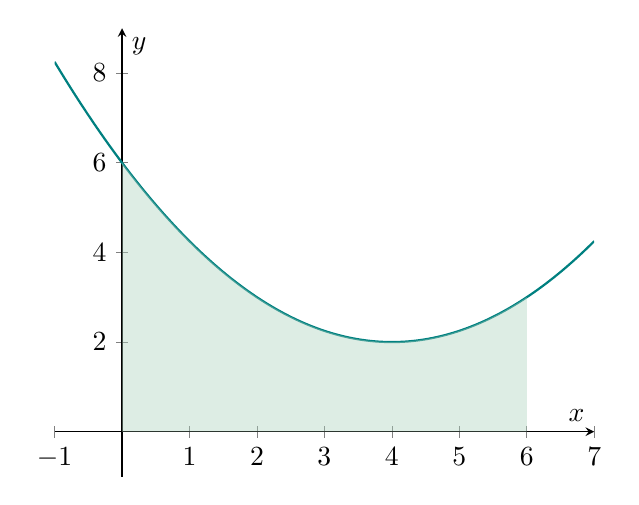
\begin{tikzpicture}
	\begin{axis}[
		axis lines = center, 
		xmin = -1, xmax = 7,
		ymin = -1, ymax = 9,
		xtick = {-4,-3,...,7,8,9},
		xlabel = $x$, 
		ylabel = $y$, 
	]
		\addplot[color = teal, thick, domain = -1:7, samples = 500] {0.25*(x - 4)^2 + 2};	
		\fill
		[
			color = SeaGreen!40,
			opacity = 0.4,
			variable = \x, 
			domain = 6:0,
			samples = 500,
		]	
			(axis cs: 0,0) -- (axis cs: 6,0) --
			plot(axis cs: \x, {0.25*(\x - 4)^2 + 2}) --  cycle;
	\end{axis}
	\end{tikzpicture}
	\caption{Areal under $f$.}
	\label{fig:opg2}
\end{figure}

\subsection*{Opgave 3}
\begin{enumerate}[label=\roman*)]
	\item Bestem arealet af det skraverede område på Figur \ref{fig:opg2}. Funktionen $f$ er givet ved
	\begin{align*}
		f(x) = \frac{2x}{\sqrt{x^2 + 4}}.
	\end{align*}
\end{enumerate}
\begin{figure}[H]
	\centering
	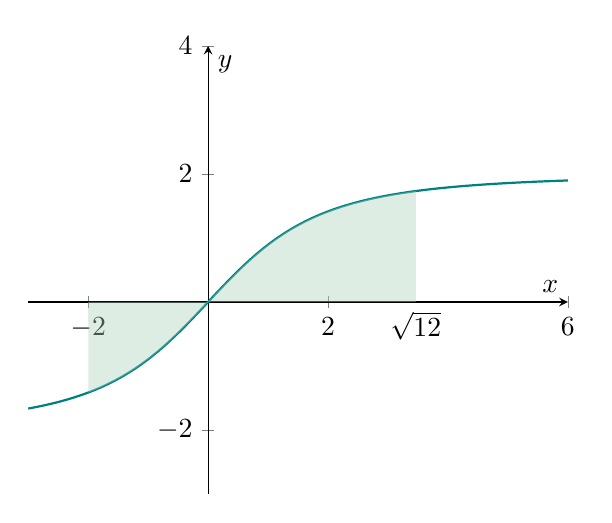
\begin{tikzpicture}
	\begin{axis}[
		axis lines = center, 
		xmin = -3, xmax = 6,
		ymin = -3, ymax = 4,
		xtick = {-6,-2,...,2,6,10},
		xlabel = $x$, 
		ylabel = $y$, 
	]
		\addplot[color = teal, thick, domain = -3:6, samples = 500] {2*x / sqrt(x^2 + 4)};	
		\fill
		[
			color = SeaGreen!40,
			opacity = 0.4,
			variable = \x, 
			domain = 3.4641:-2,
			samples = 500,
		]	
			(axis cs: -2,0) -- (axis cs: 3.4641,0) --
			plot(axis cs: \x, {2*\x / sqrt((\x)^2 + 4)}) --  cycle;
		\node[anchor = north] at (axis cs: 3.4641,0) {$\sqrt{12}$};
	\end{axis}
	\end{tikzpicture}
	\caption{Areal under $f$.}
	\label{fig:opg3}
\end{figure}


\subsection*{Udfordring 4}
\begin{enumerate}[label=\roman*)]
	\item Løs integralet
	\begin{align*}
		\int \frac{x^3}{\sqrt{x^2 + 1}} dx
	\end{align*}
	(Vink: Vælg $u = \sqrt{x^2 + 1})$
	\item Løs integralet
	\begin{align*}
		\int \frac{1}{(3t + 1)\sqrt{6t + 2}}dt		
	\end{align*}
	(Vink: Vælg $u = \sqrt{6t+2}$)
\end{enumerate}